\documentclass[12pt]{article}
\usepackage{geometry}                % See geometry.pdf to learn the layout options. There are lots.
\geometry{letterpaper}                   % ... or a4paper or a5paper or ... 
%\geometry{landscape}                % Activate for for rotated page geometry
\usepackage[parfill]{parskip}    % Activate to begin paragraphs with an empty line rather than an indent
\usepackage{graphicx}
\usepackage{amssymb}
\usepackage{subfig}
\usepackage{verbatim}
\usepackage{fullpage}
\usepackage{pstricks,pst-node,pst-tree}



\title{Breakpoints for farm field runoff}
\author{Wesley Brooks}
\date{}                                           % Activate to display a given date or no date

\usepackage{Sweave}
\begin{document}
\setkeys{Gin}{width=0.9\textwidth}    %make figures a bit wider than the Sweave default.
\maketitle








The piecewise models we use here allow a seaparate slope and intercept on either side of the breakpoint. The breakpoint chosen is the one that minimizes the residual standard error, with the condition that there must be at least four data points on both sides of the breakpoint. The p-values cited in this paper are based on an F test of the improvement in model fit between the piecewise model (with four parameters: a slope and an intercept for each line segment) and a linear model (with two parameters: one slope and one intercept covering the entire range of data).

\begin{Schunk}
\begin{Soutput}
Soil moisture breakpoints by farm:
\end{Soutput}
\begin{Soutput}
DF1: 36; p < 0.0001
DF1a: 36; p = 9e-04
DF1b: 36; p < 0.0001
DF2: 38; p < 0.0001
DF2a: 38; p < 0.0001
DF2b: 40; p < 0.0001
DF2c: 38; p < 0.0001
DF3: 36; p < 0.0001
\end{Soutput}
\end{Schunk}




\begin{figure}
    \begin{center}
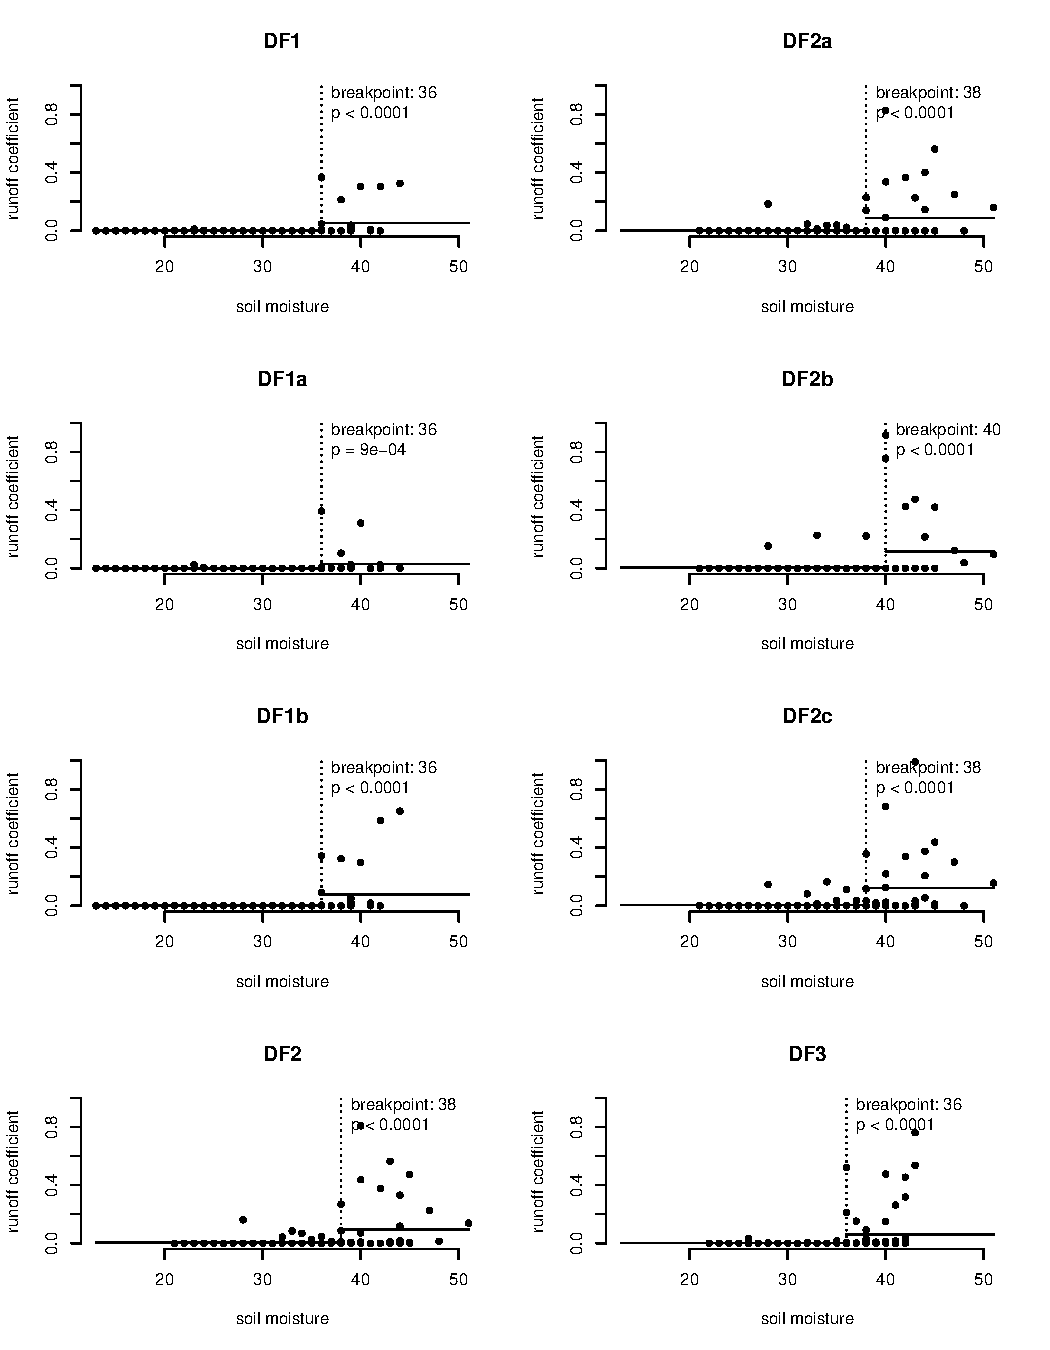
\includegraphics{runoff_constants-sm}
    \end{center}
    \caption{caption.\label{sm}}
\end{figure}


Now get the I30 breakpoints:\\

\begin{Schunk}
\begin{Soutput}
I30 breakpoints by farm:
\end{Soutput}
\begin{Soutput}
DF1: 2.3; p=p < 0.0001
DF1a: 2.3; p=p < 0.0001
DF1b: 2.3; p=p = 0.0026
DF2: 2.1; p=p < 0.0001
DF2a: 2.7; p=p < 0.0001
DF2b: 2; p=p < 0.0001
DF2c: 3.3; p=p = 0.0031
DF3: 1.2; p=p < 0.0001
\end{Soutput}
\end{Schunk}

Now split the data into two bins based on the soil moisure breakpoint (above vs. below the breakpoint) and find the I30 breakpoint in each bin:\\


\begin{Schunk}
\begin{Soutput}
Intensity breakpoints at DF1 when binned by soil moisture:
0 <= SM < 36: 1.3; p=p = 0.0424
36 <= SM < Inf: 0.6; p=p = 0.0039

Intensity breakpoints at DF2 when binned by soil moisture:
0 <= SM < 38: 1.8; p=p < 0.0001
38 <= SM < Inf: 2.2; p=p = 4e-04

Intensity breakpoints at DF3 when binned by soil moisture:
0 <= SM < 36: 1.5; p=p = 0.0114
36 <= SM < Inf: 1.6; p=p < 0.0001
\end{Soutput}
\end{Schunk}



\begin{figure}
    \begin{center}
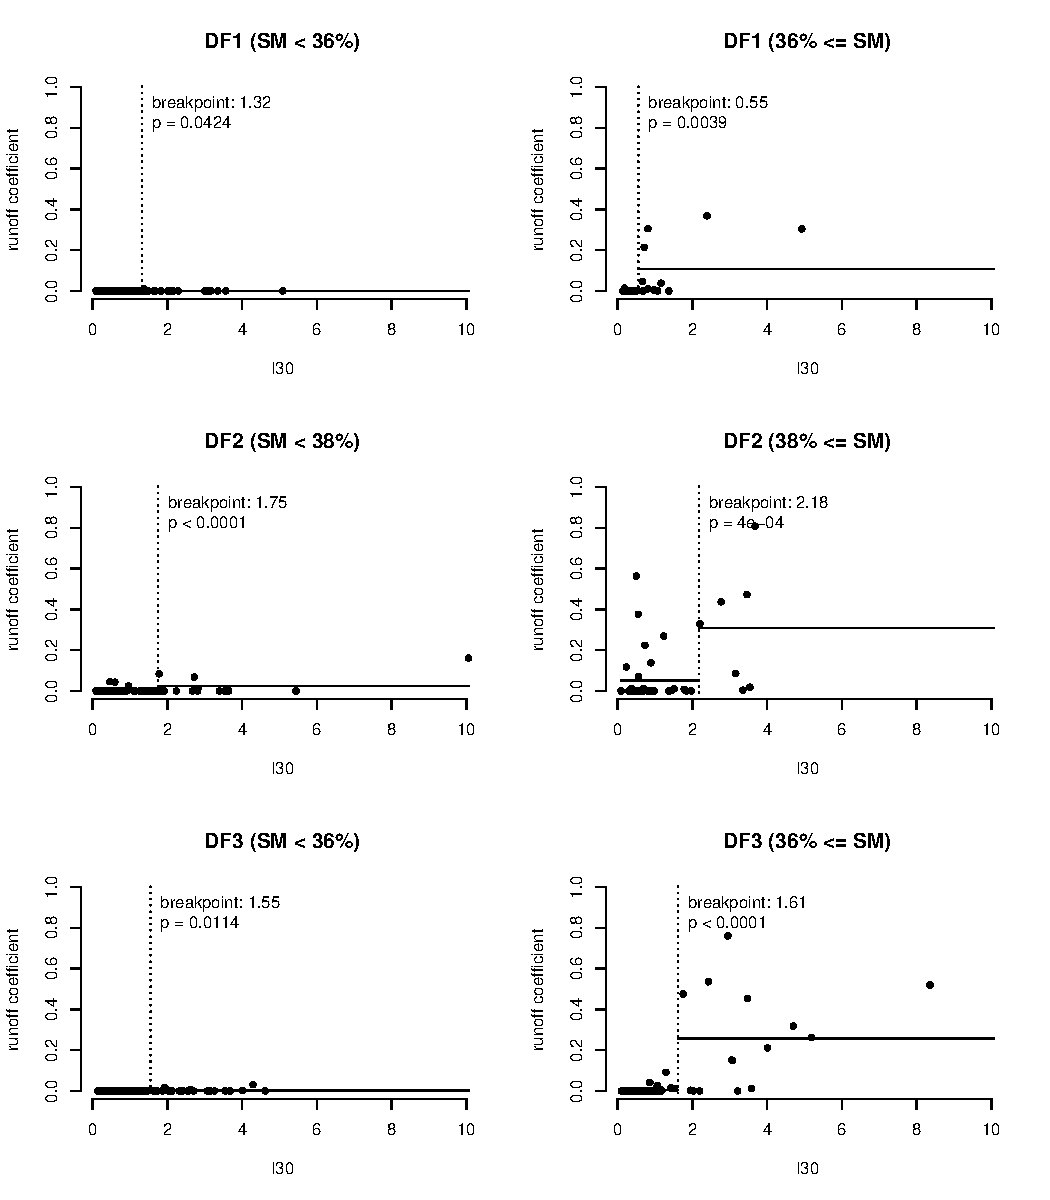
\includegraphics{runoff_constants-I30_binned}
    \end{center}
    \caption{Top row: DF1, middle row: DF2, bottom row: DF3.\label{I30_binned}}
\end{figure}


When we put the events in bins based on their antecedent soil moisture (SM: high or low), the following are the precipitation breakpoints (units are centimeters of rain):\\

\begin{Schunk}
\begin{Soutput}
Precipitation breakpoints at DF1 when binned by soil moisture:
0 <= SM < 36: 2.52; p=p < 0.0001
36 <= SM < Inf: 1.84; p=p = 2e-04

Precipitation breakpoints at DF2 when binned by soil moisture:
0 <= SM < 38: 2.07; p=p < 0.0001
38 <= SM < Inf: 2.05; p=p < 0.0001

Precipitation breakpoints at DF3 when binned by soil moisture:
0 <= SM < 36: 1.93; p=p = 7e-04
36 <= SM < Inf: 1.47; p=p < 0.0001
\end{Soutput}
\end{Schunk}





\begin{figure}
    \begin{center}
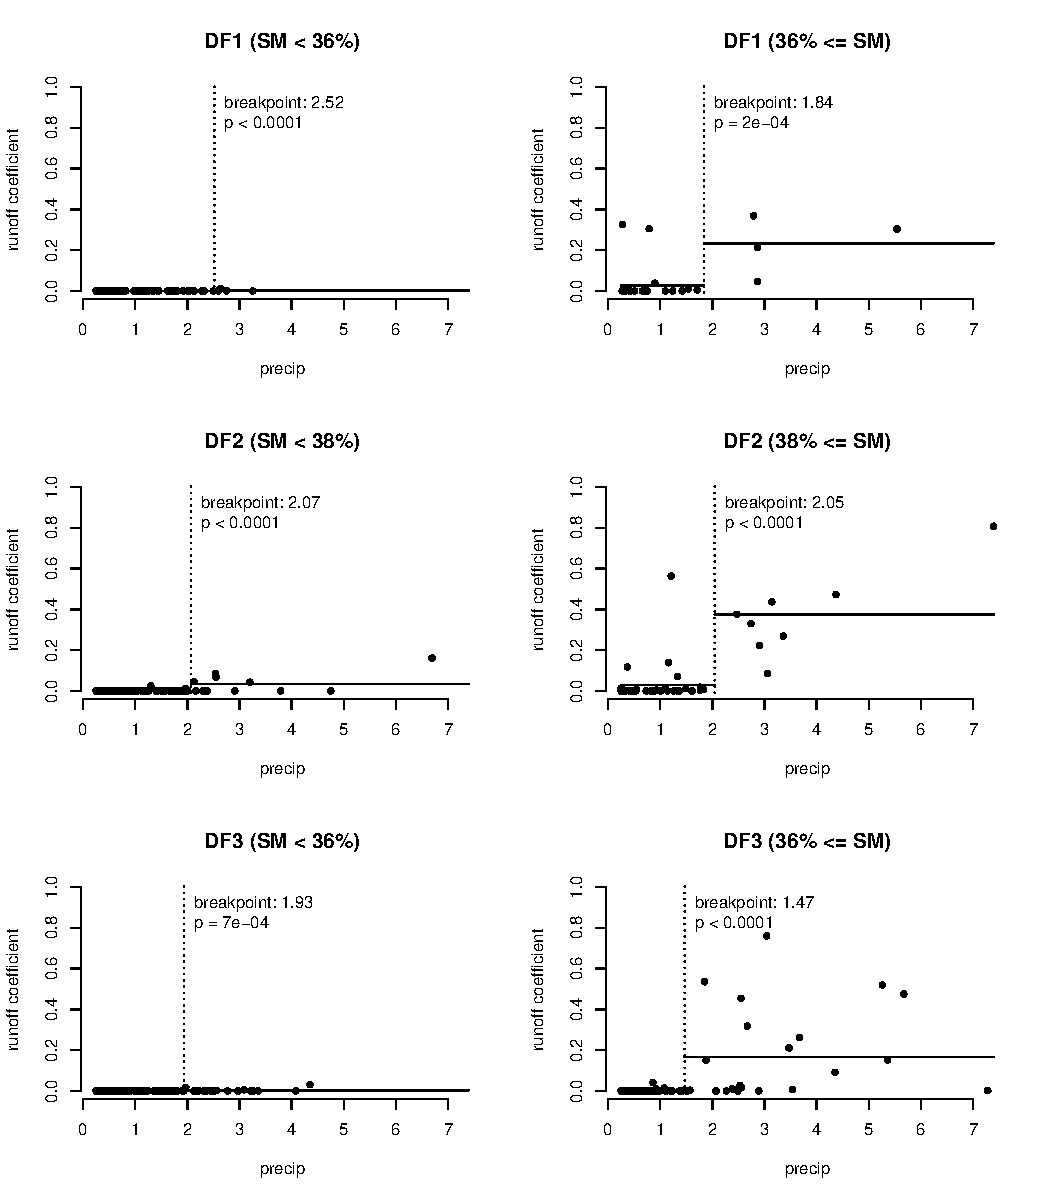
\includegraphics{runoff_constants-precip_binned}
    \end{center}
    \caption{Top row: DF1, middle row: DF1, bottom row: DF1.\label{precip_binned}}
\end{figure}

\end{document}
